%-------------------------------------------------------------------------------
%                                PREAMBLE
%-------------------------------------------------------------------------------
\documentclass[usenames,dvipsnames,svgnames,10pt,aspectratio=169]{beamer}
%
\usefonttheme{professionalfonts}
% This theme uses TIKZ: compile twice with PDFLaTeX or LuaLaTeX.
%
%  Options:
%  - [clean]:    clean slides, i.e. logos and footbar are removed
%  - [kth]:      footbar style inspierd to the official KTH template
%  - [nicewave]: a different style of wave is used (not approved by FLOW)
%
\usetheme[clean]{flow}

\usepackage{tikz}
\usetikzlibrary{arrows}
\usetikzlibrary{shapes.geometric, math, positioning, calc, patterns, angles, quotes}
\usetikzlibrary{patterns.meta,decorations.pathmorphing}

\newcommand{\semaphore}[3]{% #1: color of circle,
                           % #2: color of semicircle
                           % #3: angle of semicircle 
  \tikz[node distance=0mm,baseline]
       {
         \node (s1) [circle, fill=#1, minimum size=6mm] {};
         \node      [semicircle, fill=#2, 
           inner sep=0pt, outer sep=0pt, minimum size=3mm,
           anchor=south,
           at={(s1.center)}, rotate=#3] {};
       }
}

\usepackage[]{circuitikz}

\usepackage{pgfplots}
\usepgfplotslibrary{polar}

\usepackage{hyperref,graphicx,lmodern}
\usepackage[utf8]{inputenc}
\usepackage{media9}
\usepackage{xcolor}
\usepackage{stmaryrd}
\usepackage{nicefrac}
\usepackage{multimedia}
\usepackage{multicol}
\usepackage{upgreek}
\usepackage[]{bm}
\usepackage[]{url}
\usepackage[]{animate}
\usepackage{amsmath}

\graphicspath{{imgs/}}
\setbeamertemplate{blocks}[rounded][shadow=true]

\DeclareMathOperator*{\maximize}{maximize~}

%-------------------------------------------------------------------------------
%                                TITLE PAGE
%-------------------------------------------------------------------------------
\title[Nonlinear physics] % Short title used in footline
{
	Poincaré-Lindstedt method \\
  for periodic dynamics
}

\author[J.-Ch.~Loiseau] % Presenting author in short form used in footline
{
	\underline{Jean-Christophe Loiseau}
}
% - Give the names in the same order as the appear in the paper.
% - Underline the presenting author.

\institute[unused]
{
	\url{jean-christophe.loiseau@ensam.eu} \\
	Laboratoire DynFluid \\
	Arts et M\'etiers, France.
}
% Keep it simple, no one is interested in your street address.

% University logo(s)
\logot{\includegraphics[width=.128\paperwidth]{DynFluid_logo}}  % Top logo
\logob{\includegraphics[width=0.128\paperwidth]{ENSAM_logo}} % Bottom logo
% \logoc[{\includegraphics[width=.128\paperwidth]{limsi}}]{\includegraphics[width=.128\paperwidth]{limsi}} % Corner logo
%
% Cover image: \cvrimg{x position}{y position}{cover image}
\cvrimg{.77}{.8}{\includegraphics[width=.4\paperwidth]{cover.png}}

\date[unused]{Physique non-lin\'eaire -- 2019-2020}

\begin{document}

\titleframe	% Print the title as the first slide

%-------------------------------------------------------------------------------
%                           PRESENTATION SLIDES
%-------------------------------------------------------------------------------

\begin{frame}[t, c]{The Poincaré-Lindstedt method}{Summary}
  \begin{minipage}{.68\textwidth}
    The Poincaré-Lindstedt method is a powerful perturbative technique to approximate periodic solutions to ordinary differential equations.

    \bigskip

    By rescaling time as $\tau = \omega t$ and using power series expansions, it transforms a nonlinear system into a cascade of linear ones which we can easily solve.

    \bigskip

    The resulting approximation provides insights into the frequency shift phenomenon and harmonics generation induced by the nonlinearity.
  \end{minipage}%
  \hfill
  \begin{minipage}{.28\textwidth}
    \centering
    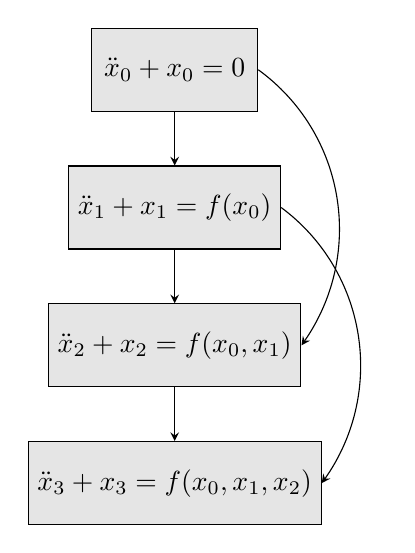
\begin{tikzpicture}[>=stealth]
      \tikzstyle{block} = [draw, fill=gray!20, rectangle, 
        minimum height=3em, minimum width=6em]

      \node [block, name=zeroth] {$\ddot{x}_0 + x_0 = 0$};
      \node [block, name=first, below of=zeroth, node distance=1.75cm] {$\ddot{x}_1 + x_1 = f(x_0)$};
      \node [block, name=second, below of=first, node distance=1.75cm] {$\ddot{x}_2 + x_2 = f(x_0, x_1)$};
      \node [block, name=third, below of=second, node distance=1.75cm] {$\ddot{x}_3 + x_3 = f(x_0, x_1, x_2)$};

      \draw[->] (zeroth) -- (first);
      \draw[->] (first) -- (second);
      \draw[->] (second) -- (third);
      \draw[->, bend right] (zeroth.east) to [out=45, in=135] (second.east);
      \draw[->, bend right] (first.east) to [out=45, in=135] (third.east);
    \end{tikzpicture}
  \end{minipage}

  \vspace{1cm}
\end{frame}

\begin{frame}[t, c]{Beyond conservative systems}{Application to the van der Pol oscillator}
  \begin{minipage}{.58\textwidth}
    Let us consider the \alert{\textbf{van der Pol oscillator}} whose governing equations are given by
    %
    \[
    \ddot{x} + x = \epsilon \left( 1 - x^2 \right) \dot{x}.
    \]
    %
    It is a canonical example of nonlinear oscillators proposed in 1927 by the Dutch electrical engineer Balthasar van der Pol.
  \end{minipage}%
  \hfill
  \begin{minipage}{.38\textwidth}
    \centering
    \includegraphics[width=\textwidth]{van_der_pol}
  \end{minipage}

  \vspace{1cm}
\end{frame}

\begin{frame}[t, c]{Beyond conservative systems}{Application to the van der Pol oscillator}
  \begin{minipage}{.58\textwidth}
    For $\epsilon > 0$, its dynamics are characterized by a limit cycle that we wish to study analytically using the Poincaré-Lindstedt method.
  \end{minipage}%
  \hfill
  \begin{minipage}{.38\textwidth}
    \centering
    \begin{tikzpicture}[>=stealth]
      \draw[->] (-2, 0) -- (2, 0) node[below] {$x$};
      \draw[->] (0, -2) -- (0, 2) node[left] {$\dot{x}$};
      
      \draw[gray!50, smooth, thick] plot file{van_der_pol_traj_1.txt};
      \draw[gray!67, smooth, thick] plot file{van_der_pol_traj_3.txt};
      \draw[gray!83, smooth, thick] plot file{van_der_pol_traj_6.txt};
      \draw[gray!100, smooth, thick] plot file{van_der_pol_traj_9.txt};
      
      \node[circle, fill=white, draw=black, inner sep=0pt, minimum size=4pt] at (0, 0) {};
    \end{tikzpicture}
  \end{minipage}

  \vspace{1cm}
\end{frame}

\begin{frame}[t, c]{Poincaré-Lindstedt method}{Application to the van der Pol oscillator}
  \begin{minipage}{.68\textwidth}
    The problem to be studied is thus the following
    %
    \[
    \left\{
    \begin{aligned}
      \ddot{x} + x & = \epsilon \left( 1 - x^2 \right) \dot{x} \\
      x(0) & = x_{\text{in}} \\
      \dot{x}(0) & = 0
    \end{aligned}
    \right.
    \]
    %
    where $x_{\text{in}}$ is the unknown initial condition and $\epsilon \ll 1$ is our control parameter.
  \end{minipage}%
  \hfill
  \begin{minipage}{.28\textwidth}
    \centering
    \begin{tikzpicture}[>=stealth]
      \draw[->] (-2, 0) -- (2, 0) node[below] {$x$};
      \draw[->] (0, -2) -- (0, 2) node[left] {$\dot{x}$};
      
      \draw[gray, smooth, thick] plot file{van_der_pol_traj.txt};
      
      \node[circle, fill=white, draw=black, inner sep=0pt, minimum size=4pt] at (0, 0) {};
    \end{tikzpicture}

    Asymptotic dynamics for $\epsilon = 0.1$
  \end{minipage}

\end{frame}

\begin{frame}[t, c]{Poincaré-Lindstedt method}{Application to the van der Pol oscillator}
  Let us rescale time as $\tau = \omega t$ such that
  %
  \[
  \dfrac{d}{dt} = \omega \dfrac{d}{d\tau}, \quad \text{and} \quad \dfrac{d^2}{dt^2} = \omega^2 \dfrac{d^2}{d\tau^2}
  \]
  %
  and use a power series expansion of the unknown frequency $\omega$, solution $x(t)$ and initial condition $x_{\text{in}}$
  %
  \[
  \begin{aligned}
    \omega & = 1 + \epsilon \omega_1 + \epsilon^2 \omega_2 + \cdots \\
    x(\tau) & = x_0(\tau) + \epsilon x_1(\tau) + \epsilon^2 x_2(\tau) + \cdots \\
    x_{\text{in}} & = A_0 + \epsilon A_1 + \epsilon^2 A_2 + \cdots
  \end{aligned}
  \]
  %
  where $x_1(\tau)$ and $x_2(\tau)$ are small corrections to the harmonic oscillator solution $x_0(\tau)$ and $\omega_1$ and $\omega_2$ are small corrections to its natural frequency.

  \vspace{1cm}
\end{frame}

\begin{frame}[t, c]{Poincaré-Lindstedt method}{Application to the van der Pol oscillator}
  \begin{minipage}{.68\textwidth}
    Introducing these expansions into our equation and regrouping by power of $\epsilon$ yields
    %
    \[
    \begin{aligned}
      \mathcal{O}(\epsilon^0) : \quad & \ddot{x}_0 + x_0 = 0 \\
      \mathcal{O}(\epsilon) : \quad & \ddot{x}_1 + x_1 = \left( 1 - x_0^2 \right) \dot{x}_0 - 2\omega_1 \ddot{x}_0 \\
      \mathcal{O}(\epsilon^2) : \quad & \ddot{x}_2 + x_2 = f(x_0, \dot{x}_0, \ddot{x}_0, x_1, \dot{x}_1, \ddot{x}_1)
    \end{aligned}
    \]
    %
    supplemented with the initial conditions
    %
    \[
    x_i(0) = A_i, \quad \dot{x}_i(0) = 0 \quad \forall i.
    \]
    %
    Once again, we trade a nonlinear system for a cascade of linear ones.
  \end{minipage}%
  \hfill
  \begin{minipage}{.28\textwidth}
    \centering
    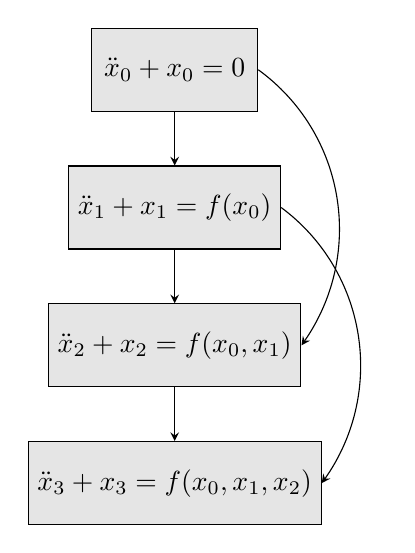
\begin{tikzpicture}[>=stealth]
      \tikzstyle{block} = [draw, fill=gray!20, rectangle, 
        minimum height=3em, minimum width=6em]

      \node [block, name=zeroth] {$\ddot{x}_0 + x_0 = 0$};
      \node [block, name=first, below of=zeroth, node distance=1.75cm] {$\ddot{x}_1 + x_1 = f(x_0)$};
      \node [block, name=second, below of=first, node distance=1.75cm] {$\ddot{x}_2 + x_2 = f(x_0, x_1)$};
      \node [block, name=third, below of=second, node distance=1.75cm] {$\ddot{x}_3 + x_3 = f(x_0, x_1, x_2)$};

      \draw[->] (zeroth) -- (first);
      \draw[->] (first) -- (second);
      \draw[->] (second) -- (third);
      \draw[->, bend right] (zeroth.east) to [out=45, in=135] (second.east);
      \draw[->, bend right] (first.east) to [out=45, in=135] (third.east);
    \end{tikzpicture}
  \end{minipage}

  \vspace{1cm}
\end{frame}

\begin{frame}[t, c]{Poincaré-Lindstedt method}{Application to the van der Pol oscillator}
  \begin{minipage}{.58\textwidth}
    The zeroth-order solution is given by $x_0(\tau) = A_0 \cos(\tau)$.
    Injecting $x_0(\tau)$ into the equation for $x_1(\tau)$ yields
    %
    \[
    \ddot{x}_1 + x_1 = A_0 \left( A_0^2 \cos^2(\tau) - 1 \right) \sin(\tau) + 2\omega_1 A_0 \cos(\tau)
    \]
    %
    which can be simplified to
    %
    \[
    \ddot{x}_1 + x_1 = 2 A_0 \omega_1 \cos(\tau) + A_0 \left( \dfrac{A_0^2}{4} - 1\right) \sin(\tau) + \dfrac{A_0^3}{4} \sin(3\tau)
    \]
    using trigonometric identities.
  \end{minipage}%
  \hfill
  \begin{minipage}{.38\textwidth}
    \centering \textbf{Trig. identity}

    \[
    \cos^2(\tau) \sin(\tau) = \dfrac{1}{4} \left( \sin(\tau) + \sin(3\tau) \right)
    \]
  \end{minipage}

  \vspace{1cm}
\end{frame}

\begin{frame}[t, c]{Poincaré-Lindstedt method}{Application to the van der Pol oscillator}
  \begin{minipage}{.68\textwidth}
    If left unchecked, the terms $\cos(\tau)$ and $\sin(\tau)$ will lead to \alert{\textbf{secular growth}}.
    We thus need to set $\omega_1$ and $A_0$ such that
    %
    \[
    \begin{aligned}
      2 A_0 \omega_1 & = 0 \\
      A_0 \left( \dfrac{A_0^2}{4} - 1 \right) & = 0
    \end{aligned}
    \]
    %
    to avoid this unphysical behaviour.
    This leads to $\omega_1 = 0$ and $A_0 = 2$.
  \end{minipage}%
  \hfill
  \begin{minipage}{.28\textwidth}
    \centering
    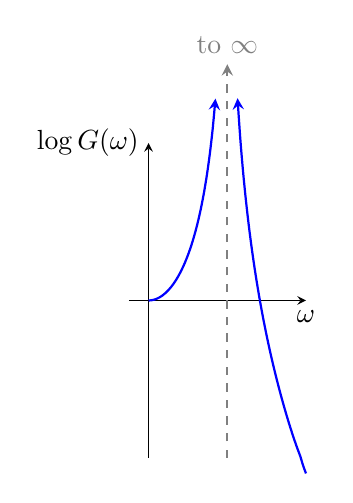
\begin{tikzpicture}[>=stealth]
      \draw[->] (-0.25, 0) -- (2, 0) node[below] {$\omega$};
      \draw[->] (0, -2) -- (0, 2) node[left] {$\log G(\omega)$};

      \draw[->, blue, thick, smooth, domain=0:0.85, variable=\x] plot (\x, {ln(1/(1-\x*\x)^2)});
      \draw[<-, blue, thick, smooth, domain=1.13:2, variable=\x] plot (\x, {ln(1/(1-\x*\x)^2)});

      \draw[->, dashed, gray, smooth, thick] (1, -2) -- (1, 3) node[above] {to $\infty$};

    \end{tikzpicture}
  \end{minipage}

  \vspace{1cm}
\end{frame}

\begin{frame}[t, c]{Poincaré-Lindstedt method}{Application to the van der Pol oscillator}
  \begin{minipage}{.68\textwidth}
    At order $\mathcal{O}(\epsilon)$, the equation reduces to
    %
    \[
    \ddot{x}_1 + x_1 =  2 \sin(3\tau)
    \]
    %
    whose general solution is given by $x_1(\tau) = ??$.
    Note that $A_1$ is still undetermined and one needs to go to order $\mathcal{O}(\epsilon^2)$ to determine it.
  \end{minipage}%
  \hfill
  \begin{minipage}{.28\textwidth}
    \centering
    \begin{tikzpicture}[>=stealth]
      \draw[->] (-0.25, 0) -- (2.25, 0) node[below] {$\epsilon$};
      \draw[->] (0, -0.25) -- (0, 2.25) node[left] {$\omega$};

      \draw[red, thick, dashed] (0, 1) -- (2, 1) node[above] {$\omega_0$};

    \end{tikzpicture}
  \end{minipage}

  \vspace{1cm}
\end{frame}

\begin{frame}[t, c]{Poincaré-Lindstedt method}{Application to the van der Pol oscillator}
  \begin{minipage}{.68\textwidth}
    Continuing this process to $\mathcal{O}(\epsilon)$ leads to the second-order frequency correction
    %
    \[
    \omega_2 =  \dfrac{7}{16}
    \]
    %
    as well as to the condition $A_1 = 0$.
    Our first-order approximation thus reads
    %
    \[
    x(t) = 2 \cos(\omega t) + \epsilon \left( \dfrac{3}{4} \sin(\omega t) - \dfrac{1}{4} \sin(3\omega t) \right) + \mathcal{O}(\epsilon^2)
    \]
    %
    with $\omega = 1 + \dfrac{7\epsilon^2}{16} + \mathcal{O}(\epsilon^4)$.
    Once again, nonlinearity causes a \alert{\textbf{frequency shift}} and the generation of \alert{\textbf{high-order harmonics}}.
  \end{minipage}%
  \hfill
  \begin{minipage}{.28\textwidth}
    \centering
    \begin{tikzpicture}[>=stealth]
      \draw[->] (-0.25, 0) -- (2.25, 0) node[below] {$\epsilon$};
      \draw[->] (0, -0.25) -- (0, 5.25) node[left] {$\omega$};

      \draw[red, thick, dashed] (0, 1) -- (2, 1) node[below] {$\omega_0$};
      \draw[blue, thick, smooth, domain=0:2, variable=\x] plot (\x, {(1 + 7*\x*\x / 1000)}) node[above] {$\omega$};
      \draw[blue, thick, smooth, domain=0:2, variable=\x] plot (\x, {3*(1 + 7*\x*\x / 1000)}) node[above] {$3\omega$};

    \end{tikzpicture}
  \end{minipage}

  \vspace{1cm}
\end{frame}

\begin{frame}[t, c]{Poincaré-Lindstedt method}{Application to the van der Pol oscillator}
  \centering
  \includegraphics[width=.8\textwidth]{van_der_pol_spectrum}
\end{frame}

\begin{frame}[t, c]{Poincaré-Lindstedt : the van der Pol oscillator}{Summary}
  \begin{minipage}{.68\textwidth}
    The Poincaré-Lindstedt method is a powerful perturbative technique to approximate periodic solutions to ordinary differential equations.

    \bigskip

    For $\epsilon < 0$, the only attractor is a stable fixed point.
    As $\epsilon$ becomes positive, the dynamics settles on a constant-amplitude limit cycle.

    \bigskip

    By design, the Poincaré-Lindstedt method cannot however capture transient effects.
    We'll need another technique for that purpose.
  \end{minipage}%
  \hfill
  \begin{minipage}{.28\textwidth}
    \centering
    \begin{tikzpicture}[>=stealth]
      \draw[->] (-2, 0) -- (2, 0) node[below] {$x$};
      \draw[->] (0, -2) -- (0, 2) node[left] {$\dot{x}$};
      
      \draw[gray, thick] plot file{van_der_pol_traj_bis.txt};
      
      \node[circle, fill=white, draw=black, inner sep=0pt, minimum size=4pt] at (0, 0) {};
    \end{tikzpicture}
  \end{minipage}

\end{frame}

\end{document}
